\section{Methods}

\subsection{Experimental procedures}

\subsubsection{Dish preparation}
First, WillCo glass dishes ($\O$30 mm, WillCO Wells) were rinsed with acetone,
isopropanol and ultra pure Water (Millipore Milli-Q System, 18M$\Omega$), then
dried with a nitrogen gun. Next, double sided adhesive rings were used to
attach WillCo glass dishes to polystyrene dish frames. The assembled dishes were
placed in a larger plastic dish with tape stripes preventing surface adhesion
between dishes.

% respectively, and dried with nitrogen gun. Finally, the cover slip
% was sealed off to the bottom of the dish. For the experimental groups, small
% plastic Petri dishes ($\O$40 mm) were coated with PDMS by adding approximately
% 250 $\mu$L of PDMS to the centre of the dish without forming any bubbles,
% spin-coating at 1500 rpm for 60 secs and then curing for 2 hours at 80
% $^{\circ}$C. The dishes were placed inside a bigger Petri dish to make the
% handling easier. A strip of tape was added to the bottom of the big Petri dish
% in order to prevent glass bottom dishes sticking. Prior to coating, all the
% dishes were sterilised under UV light for 4 hours or 2 hours at 80 $^{\circ}$C.

\subsubsection{Poly-D-Lysine \& laminin coating}
The assembled glass dishes were coated using 1 ml Poly-D-Lysine (PDL) solution
(56 $\upmu$g/ml), incubating for 1-2 hours at room temperature. The solution was
prepared using 1 ml of thawed up PDL stock (P7280, Sigma-Aldrich), and 8 ml of
phosphate buffered saline (PBS) (10010015, Gibco, Thermo Fisher Scientific,
Switzerland). After incubation, the PDL solution was removed and the dishes were
washed 2 times with PBS, and once with deionized (DI) water  to avoid salt
crystal formation. \\

% PDL coating solution  was prepared by adding 1 mL of PDL (P7280, Sigma-Aldrich)
% stock was thawed and mixed with 8 mL of sterile PBS (10010015, Gibco, Thermo
% Fisher Scientific, Switzerland). 2 mL of the PDL solution was added to each dish
% and incubated at 4 $^{\circ}$C over night. The PDL solution was washed 3x with
% PBS and then once 1x with sterile DI water. PDL solution should be washed
% completely since non-physisorbed PDL polymer fragments can be toxic for the
% neurons. \cite{shin2012microfluidic} \cite{lau2013cell}) Finally, the dishes
% were dried in the hood for 1 hr. 

Subsequent to PDL application, dishes were coated with 10 $\upmu$g/ml laminin.
This solution was prepared by slowly thawing 50 $\upmu$l aliquots on ice, then
adding 5 ml of Neurobasal$\rm^{TM}$ plus (A3582901, Gibco). Between 300-800
$\upmu$l laminin solution was applied to cover the whole surface of the glass
dish. After 24h incubation at 37 $^{\circ}$C, laminin solution was removed and
the dishes were washed 1 time with PBS, and 2 times with DI water.


% In order to prepare the laminin coating solution of concentration 10 $\mu$g/mL,
% 50 $\mu$L laminin (1 mg/mL) stock was thawed on ice to prevent gelation and was
% later added to 5 mL Neurobasal$^{TM}$ plus medium (A3582901, Gibco). For
% experimental groups involving laminin coating, the surface of dish was covered 2
% mL with the laminin solution after the PDL washes and incubated over night at 37
% $^{\circ}$C incubator or at 4 $^{\circ}$C for 48 hours. After the incubation,
% laminin solution was washed 1x with PBS and 2x with sterile DI water to avoid
% formation of salt crystals.


\subsubsection{PDMS micro structure design, fabrication \& mounting}
\label{pdms structures assembly}
PDMS micro structures were designed in a multi stage computer aided design (CAD)
process. This was necessitated by the vast number of design motifs investigated
in this study. Although not primarily intended for 2D CAD, Fusion360 (Autodesk,
San Rafael, California) was used in the initial design stage. Fusion360 was
chosen because of its powerful version control and design history system,
enabling the natural integration of design variables into the CAD workflow.
Specific elements in different PDMS designs were inserted as separate components
such that they could be updated independently from the base designs; for example
the commonly used 2-joint motif. Single PDMS designs were then exported as
\verb|.dxf| files by projecting extruded bodies to 2D sketches. Importantly, the
projection link had to be deleted to export valid \verb|.dxf| files. The single
PDMS designs were imported to AutoCAD (Autodesk, San Rafael, California) to
define fabrication mask layers and arrange designs on the wafer. Finally, the
wafer design was exported as a \verb|.dxf| file and imported from KLayout where
the final \verb|.gds2| file was generated. The wafer and PDMS designs were
fabricated by Wunderlichips (Switzerland) employing standard soft lithography
(for details see \cite{forro}). \\

The PDMS membrane delivered by Wunderlichips was separated into independent PDMS
structures on a laser cutter (Speedy300, Trotec, Switzerland) using 8 \% power
at 14 cm/s. Subsequently, the structures were thoroughly rinsed with 70 \%
ethanol. For a subset of experiments, a PDMS frame was laser cut from 5mm thick
cured PDMS. Using uncured PDMS, it was attached on the micro structure to
enclose the output channel area. After curing for 1h at 80$^{\circ}$C, they were
picked up with a pair of surgical forceps and slowly placed on the coated glass
dishes (see above). Importantly, prior to mounting, a thin film of DI water was
put on the glass dishes to facilitate mounting without enclosed air bubbles. As
the last dish preparation step, RGC medium (see composition in Table
\ref{rgcmedium}) was added and the dishes were desiccated for 30-60 minutes to
remove air from the PDMS micro channels.

\begin{table*}
    \begin{adjustbox}{max width=\textwidth,center}
        \begin{tabular}{@{}rrrrrrrr@{}}
            \toprule
            & & & & & Component & Volume [ml] & Stored at [$^{\circ}$C] \\
            \midrule
            & & & & & Neurobasal Plus (Gibco, A3582901)               & 237.5    &   4\\
            & & & & & DMEM (Gibco 11960                               & 237.5    &   4\\
            & & & & & Glutamax                                        & 5        &   4\\
            & & & & & Sodium Pyruvate (100mM, Gibco 11360-070)        & 5        &   4\\
            & & & & & Antibiotic-Antimycotic (100x, Gibco 15240096)   & 5        & -20\\
            & & & & & N2 Supplement                                   & 5        & -20\\
            & & & & & B27+ (50x)                                      & 10       & -20\\
            & & & & & N21 Supplement (50x, R$\&$D Systems AR008)      & 10       & -20\\
            & & & & & NAC Stock (5 mg/mL)                             & 0.5      & -20\\
            & & & & & Forskolin Stock (4.2 mg/mL)                     & 0.5      & -20\\
            & & & & & BDNF Stock (50 $\mu$g/mL, Preprotech 450-02)    & 0.5      & -20\\
            & & & & & CNTF Stock (10 $\mu$g/mL, Preprotech 450-13)    & 0.5      & -80\\
            & & & & & NGF 7S Stock (10 $\mu$g/mL, final 10 ng/mL)     & 0.5      & -80\\
            & & & & & GNDF (10 ng/mL)                                 & 0.5      & -20\\
            \bottomrule
        \end{tabular}
    \end{adjustbox}
    \caption[RGC medium composition]{RGC medium composition. This medium was
            used throughout for culturing RGC neurons.}
    \label{rgcmedium}
\end{table*}

% Briefly, a negative SU8 photoresist (SU8 3000 Series, MicroChem, USA) was spin
% coated on a silicon wafer, selectively cross-linked by passing UV light through
% a photomask in two consecutive layers, and the uncrosslinked photoresist
% dissolved in mr-Dev 600 (Microresist Technologies, Germany) to create a mold for
% the PDMS devices. Next, the mold was treated with perfluoro-octyl
% trichlorosilane (AB111444, ABCR, Germany) in a desiccator chamber with low
% vacuum applied. PDMS (Sylgard 184, Dow Corning) was then spin coated, cured
% overnight at 70 °C , peeled off and transferred to a clean container.
% Uncrosslinked PDMS was extracted from the devices by immersing them in iso-
% propanol for a minimum 1 h to improve cell viability (Millet et al., 2007).

% \subsubsection{Primary Cell Culture (EYLUL)}
% All cell culture experiments were performed using primary cells from cortices
% and eyeballs of E18 embryos of time-mated pregnant rats . Animal experiments were approved by the Cantonal Veterinary Office
% Zurich.


% \subsubsection{Retina Dissections (EYLUL)} 
%  Dissection instruments, microscalpels, scissors and forceps were sprayed with
%  70 $\%$ ethanol prior to dissections. The retina dissections were performed
%  under a benchtop microscope (DFC420C with 4X magnification, Leica, Germany) in
%  a Petri dish filled with hibernate medium. Retinas were dissected out from
%  whole eyeball. Firstly, all the tissue around the eyeballs was removed. The
%  eyeballs were pinched along the cornea-sclera edge and cornea with forceps on
%  both sides and gently pulled apart to cut open and isolate the retina. After
%  gently removing the lens, the retina was later cut into square explants of
%  around size 500 $\mu$m X 500 $\mu$m. After the dissections, the ~100 $\mu$L
%  dissected retina explants were transferred to a small Eppendorf tube and tagged
%  with an adeno-associated virus (AVV) encoding for the mRuby virus
%  (scAAV-DJ/2-hSyn1-chl-mRuby3-SV40p(A)). To do so, mRuby virus vial was thawed
%  on ice and 1 $\mu$L was added to the explants. The explants were incubated with
%  mRuby on ice for 1 hour.

% \subsubsection{AggreWell\textsuperscript{\texttrademark} Preparation and Cell Dissociation (EYLUL)}
% AggreWell\textsuperscript{\texttrademark} plate preparations to produce
% reproducible spheroids and cell dissociation were performed in parallel.
% AggreWell\textsuperscript{\texttrademark} 800 microwell culture plates were
% prepared by adding 500 $\mu$L of AggreWell\textsuperscript{\texttrademark}
% rinsing solution to the needed wells in order to prevent cell adhesion and
% promote spheroid formation. 

% The plate was then balanced by adding 300 $\mu$L of
% DI water to each well of a standard well plate and centrifuged at 2000 x g for 5
% minutes. The plate was examined under the microscope and check for bubbles. If
% there are trapped bubbles in the micro-well, the centrifuge procedure was
% repeated again. 

% Afterwards, the AggreWell\textsuperscript{\texttrademark}
% rinsing solution was aspirated and each well was rinsed with 2 mL of warm
% Neurobasal medium. 1 mL of complete medium was added to each well and the plate
% was kept in the incubator until cell dissociation was completed. 


\subsubsection{Retina dissection}
\label{dissection}
Animal experiments were performed with highest of care maximizing animal welfare
and following 3 R. The approval was obtained from Cantonal Veterinary Office
Zurich, Switzerland under license SR 31175 - ZH048/19. E18 time-mated pregnant
rats (Janvier Laboratories, France) were sacrificed and embryonic eyes were
collected in Hibernate medium on ice. Before retinal dissection, instruments
were disinfected using 70\% ethanol. Under a benchtop microscope (DFC420C with
4X magnification, Leica, Germany), eyeballs were pierced near the ciliary
muscles using a sharp pair of forceps. This opening was carefully extended by
inserting a second pair of forceps on which the sclera was subsequently striped
off. Retinas were collected in Hibernate medium on ice after gently removing the
lens and hyaloid vasculature.

\subsubsection{Spheroid creation}
To create RGC and thalamus spheroids, first, 500 $\upmu$l of
AggreWell\textsuperscript{\texttrademark} rinsing solution was added to the
AggreWell\textsuperscript{\texttrademark} 800 microwell plates. To ensure the
absence of air bubbles in the microwells, the plate was centrifuged at 2000 g
for 5 minutes or until no air bubbles were observed. Finally, the rinsing
solution was washed away with Neurobasal medium and 1 ml of RGC medium was added
to each of the micro wells. \\

For retina and thalamus dissociation, first, a solution was prepared by
dissolving 50 mg BSA and 90.08 mg glucose in 50 ml of sterile PBS. 5 ml of this
solution were vortexed with 2.5 mg Papain. After 30 minutes of incubation at
room temperature, the Papain solution was filtered using a 0.2 $\upmu$m sterile
filter and 5 $\upmu$l DNAse were added. Tissues were dissociated by first
incubating them for 15 minutes at 37 $^{\circ}$C in 5 ml of this Papain
solution. After 15 minutes, the Papain solution was carefully removed without
disturbing the pallet. In three cycles, 5 ml of warmed Neurobasal medium were
added, incubated for 3 minutes, then removed again. To suspend the retinas, 2 ml
of RGC medium were added and repeatedly pipetted up and down using a pipette
boy. After cell straining with a 40 $\upmu$m filter, the number of viable cells
was determined using a Trypan Blue stain on a hemocytometer. To create spheroids
of 3000 cells, the appropriate cell concentration to fill 300 micro wells was
calculated and prepared. In order to obtain constant volumina across
experiments, wells were filled up to 2 ml using RGC medium. Lastly, to
color-label the spheroids, one $\upmu$l of mRuby virus
(scAAV-DJ/2-hSyn1-chl-mRuby3-SV40p(A), hereafter called RFP) or GFP virus
(scAAV-DJ/2-hSyn1-chI-EGFP- SV40p(A)) was added for adeno-associated virus (AAV)
mediated transduction. The AggreWell\textsuperscript{\texttrademark} plate was
then centrifuged at 100 g for 3 minutes to fill the microwells with cells. After
confirming even cell distribution and expected spheroid sizes, the plate was
placed in the incubator at 37 $^{\circ}$C with 5$\%$ CO$_{2}$ for 16-20 hours. 

\subsubsection{Seeding PDMS micro structures}
To remove the virus before seeding, spheroids were pipetted out of the
AggreWell\textsuperscript{\texttrademark} plate into a small petri dish and
carefully washed in Neurobasal three times. Under the benchtop microscope,
around 50 spheroids were pipetted from the petri dish into the prepared micro
structure dish (see \ref{pdms structures assembly}). They were then carefully
placed in the appropriate location within the PDMS micro structures using a pair
of micro scalpels. Timelapse structures were either additionally seeded with
thalamus spheroids or small thalamic tissue pieces were placed on top of the
PDMS micro structure output channel. After 10 minutes of seeding, the culture
was transferred back to the incubator for 5 minutes to recover the pH. Once all
seeding spots were filled, the culture was placed in the incubator at 37
$^{\circ}$C with 5  \% CO$_{2}$. Half the RGC medium was exchanged every 3-4
days.

\subsubsection{Timelapse recording \& image acquisition}
\label{imagingsettings}
Both timelapse,- and single images were recorded on an inverted confocal laser
scanning microscope (CLSM) (FLUOVIEW FV3000, Olympus). Timelapse recordings were
performed using a 20x objective, 800 $\upmu$m pinhole, a gain of 580-600 V, and
laser power of 0.8-1 \%. The axonal growth in each of the approx. 40 PDMS micro
structures was captured by 2 x 4, 1024x1024 tile scans, resulting in an optical
resolution of 0.49 $\upmu$m, and a pixel size of 0.62 $\upmu$m. Absorption and
emission spectra of fluorescent markers were set according to the manufacturers
recommendations. To maintain cell viability throughout the recording, the
integrated incubator chamber was setup to 37 $^{\circ}$C with 5 \% CO$_{2}$.
Fast solid state storage media was used to prevent a frame rate bottleneck from
an insufficiently fast network connection. \\
Single images were acquired under the same settings, except that a 10x objective
was used. This resulted in an optical resolution of 0.88 $\upmu$m and a pixel
size of 1.24 $\upmu$m. 

\subsection{Data analysis}
\subsubsection{Timelapse datasets}
This work incorporates three PDMS micros structure timelapse recordings that
were acquired at different timepoints. Accordingly, the data used in this work
is based on three experiments, where each experiment was performed with 8-14 rat
embryos (compare \ref{dissection} for details). One of the three timelapses was
solely obtained for generating model training data, thus the presented results
are based on two experiments with a total of 16-28 biological replicates. A
summery of timelapse datasets is given in Table \ref{datasets_table}. \\

We treat each half of a PDMS micro structures as independent samples, as all
designs are strictly symmetric around the output channel. Given that the two
experiments included each design in duplicate, a maximum of 8 samples per design
were obtained. However, since fabrication failure within designs, bad tracking
performance, and overly strong undergrowth led to discarding samples, few
designs are limited to a sample size of n = 4.

\begin{table*}[h!]
\begin{adjustbox}{max width=\textwidth,center}
    \begin{tabular}{@{}rrrrrrrrrrrr@{}}
    \toprule
    & Acquired & Setup  & T [min] & n frames & Length [days] & Model usage\\
    \midrule
    \vspace{2mm}
    Dataset1 & 20.12.20 & 1 design  &  40 & 37  & 1   & Training\\
    Dataset2 & 27.08.21 & 2 designs, chamber  &  31 & 210 & 4.5 & Training\\ 
    \vspace{2mm}
    Dataset3 & 27.10.21 & 18 designs, chamber &  31 & 210 & 4.5 & Inference\\
    Dataset4 & 07.10.21 & 21 designs, stomachs &  32 & 242 & 5.4 & Inference\\
    \bottomrule
    \end{tabular}
\end{adjustbox}
\caption[Overview of timelapse recording data]
        {Overview of timelapse recording data.
         \textit{n designs} refers to the number of unique PDMS micro structure
         designs composing the dataset. \textit{Chamber} setups employed large  
         thalamic tissue pieces enclosed by a PDMS frame for concentrated
         attraction cues (see \ref{pdms structures assembly} for details).
         \textit{Stomach} setups omitted PDMS frames and instead seeded a
         thalamic spheroid in the target well (see Figure
         \ref{I_thal_innervation} C). T refers to the temporal period of the
         recording. White space between rows indicates different experiments.}
\label{datasets_table}
\end{table*}

\subsubsection{Initial timelapse processing}
The proprietary \verb|.oir| files produced by the CLSM were converted to three
dimensional \verb|.tif| files using Python's \verb|bioformats| package, which
relies on a java virtual machine implemented within the \verb|javabridge|
package. Additionally, \verb|.tif| frame sequences were rendered to \verb|.mp4|
video using \verb|scikit-image| and \verb|open-cv| (Suppl. Figure
\ref{SF_intial_tl_preprocessing} A). These videos were used for initial
evaluation of the timelapse, validating for example absence of strong
undergrowth and artifacts. The transmission channel of each PDMS micro structure
timelapse was then loaded into napari, a python based n-dimensional image viewer
\parencite{Sofroniew2021}. Using \verb|skimage.filters| to segment the micro
channels in the PDMS designs, edge magnitude was detected with \verb|prewitt()|,
gaussian smoothing was performed with \verb|gaussion()| ($\rm\sigma=1$),
thresholding was done with \verb|threshold_otsu()|, and finally, the
segmentation was cleaned up using \verb|skimage.morphology.binary_closing()|
(diameter = 4) (Suppl. Figure \ref{SF_intial_tl_preprocessing} B). Subsequently,
the segmentation of the PDMS micro channels was manually cleaned up, mainly
using the bucket tool to fill areas enclosed by detected edges. To remove
patches in the mask, the target point of the PDMS design was labelled and used
as the origin to perform \verb|skimage.segmentation.flood()|. To recognize
specific axon locations, both the final output channel and the first 100
$\rm\upmu m$ of the channels exiting the source wells were segmented and saved
as binary masks (Suppl. Figure \ref{SF_intial_tl_preprocessing} C).

\subsubsection{Axon growth cone labelling}
The axon growth cone tracking model was trained using Dataset1, and Dataset2
which included timelapse recordings of three unique PDMS designs (compare Table
\ref{datasets_table}). The labelling of these three image sequences was
performed by one human expert using the napari image viewer. The workflow for 
obtaining the four dimensional label of
 \verb|FrameID| - \verb|AxonID| - \verb|X coordinate| - \verb|Y coordinate| was
as follows:
\vspace{2mm}
\begin{enumerate}
    \item Load timelapse sequence.
    \item Create empty set of axon identities.
    \item Inspect short time slice of 3-6 frames for distinct, coherently moving
    blob.
    \item Identify axon identity by its growth cone.
    \item Trace axon identify over adjacent frames until unidentifiable.
\end{enumerate}
\vspace{2mm}
In the scenario where two separate growth cones converge forming a single
observable growth cone, one of the two identities was arbitrarily chosen to be
continued while the other one was terminated. Hence, the underlying number of
axons for a given growth cone label may be larger than one. It should also be
considered that there is some degree of uncertainly in the ground truth labels.
Especially when the PDMS micro channels become largely filled, distinguishing
between GFP-protein trafficking along existing axons versus new growth cones
becomes challenging. The annotations here were consistently done more
conservatively, weighting the avoidance of false positives higher than missing
true positives. Following this conservative labelling methodology, an axon
identity was only considered if it appeared over more than three frames. From
three concatenated PDMS micro structure timelapses, 300 growth cones were
identified over N=327 frames where the average axon identity lifetime was 24
frames.  Four labelled example frames are shown in Suppl. Figure
\ref{SF_training_data}, and an overview of the axon identify lifetime is given
in Suppl. Figure \ref{SF_methods_expl} A.

\subsubsection{Timelapse data preprocessing}
The CLSM \verb|12bit| gray scale intensity values saved as 
\verb|16bit unsigned integers| were first converted to a scale of 0 to 1 using
\verb|skimage.util.img_as_float()|. For image sequences that had an offset in
the intensity profile, this offset was subtracted such that the minimal
intensity was always 0. Next, the segmentation of the micro channels was used to
mask the image sequence (see Suppl. Figure \ref{SF_intial_tl_preprocessing} C
for an example mask). The resulting initial distribution of intensity values for
two example training and inference frames are shown in  Suppl. Figure
\ref{SF_image_preproc} A top left. In the next step, intensity values below
threshold = 0.00083 were clipped and set to 0 (top right). Then, the intensity
profile $I_{in}$ was stretched using \verb|skimage.exposure.adjust_log()|
function with a gain  \textit{g} = 1 which transformed the distribution
according to formula \ref{formula_log_adjust} (bottom left). 

\begin{equation}
    I_{out} = g*log(1 + I_{in})
    \label{formula_log_adjust}
\end{equation}
\vspace{0.1mm}

Finally, the intensity distribution was divided by the global standard deviation
across the entire training image sequence, ensuring unit variance in the model
input data (Suppl. Figure \ref{SF_image_preproc} A, bottom right). Both
frame-wise, and mean-based standardizations were omitted since their application
resulted in decreased detection performance. The intensity distributions from
train- and inference data do not overlap in Figure \ref{SF_image_preproc} A
because the sparsity differs vastly across frames. Train intensity values do not
increase from $\rm t_0$ to $\rm t_N$ because $\rm t_N$ corresponds to a
different timelapse video (Dataset2) which is more sparse than $\rm t_0$
(Dataset1).


\subsubsection{Growth cone detection model}
\label{modeldescription}
\paragraph{Temporal context frames}
The growth cone detection model implemented in \verb|PyTorch| follows the
general approach of YOLO \parencite{yolo} where the detections are obtained by a
single pass through the network (Figure \ref{M_preprocessing} A). The first
aspect in which it deviates from the original is that instead of inputting an
RGB image, the network receives a temporal stack of five gray scale images.
Concretely, to detect growth cones at frame $\rm t_0$, frame $\rm t_{-2},
t_{-1}, t_{0}, t_{1}, t_{2}$ are fed into the network. This architecture aims to
imitate the strategy of human labelling: by inspecting single frames, growth
cone identification is highly uncertain; only when scanning sequences of frames,
coherently moving blobs of particular shape and dynamics can be linked to growth
cones and thus an axon identity. To always provide full temporal context, frame
$t_{0}, t_{1}, t_{N-1}, t_{N}$ were omitted from detecting growth cones in the
image sequence. Computing the motion between frames manually by subtraction
yielded decreased detection performance over the implicit approach of passing
temporal context frames. An illustration of the motion computation is shown in
Figure \ref{M_preprocessing} B.

\begin{figure}[h!]
    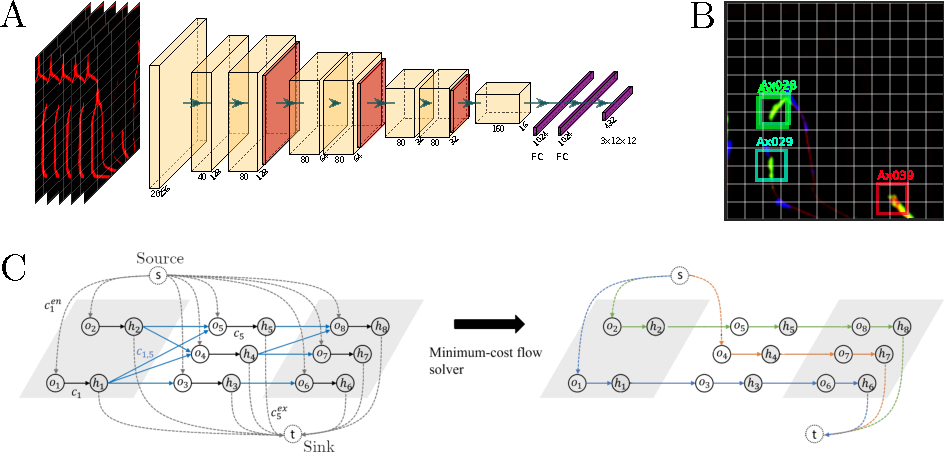
\includegraphics{M_preprocessing.pdf}
    \caption[Growth cone tracking model overview]{Growth cone tracking model
             overview. \textbf{A} CNN architecture. Each yellow block in
             represents a sequence of 2D-convolution, batch normalization
             \parencite{BN}, and Leaky ReLU \parencite{leakyrelu}. Orange layers
             stand for maximum pooling operations. FC stands for fully connected
             layers. \textbf{B} Example tile illustrating the YOLO label format.
             Each grid box can be predicted to contain a growth cone. In this
             example, 4 of 12 x 12 grid boxes are positive. Green colors in the
             tile represent positive motion (pixel intensity increased from
             frame $\rm t_0$ to $\rm t_1$), blue represents negative motion.
             Grid box size = 26 $\rm \upmu m$. \textbf{C} Minimum cost flow
             optimization illustration adopted from \parencite{MCF}. Frames are
             illustrated in gray and white background, detections within a frame
             are represented by a pre- ($o_i$), and post ($h_i$) node. Blue
             edges on the left represent costs between detections in adjacent
             frames. Coloured edges on the right indicate identity assocications
             after solving the graph. 
             } 
    \label{M_preprocessing}
\end{figure}

\paragraph{Tiling}
Each yellow block in Figure \ref{M_preprocessing} A represents a sequence of
2D-convolution, batch normalization \parencite{BN}, and Leaky ReLU
\parencite{leakyrelu}. Orange layers stand for maximum pooling operations. As
performing detection on the original resolution of 3868 x 1972 was
computationally intractable, the timelapse frames were split into 512 x 512
tiles (see Figure \ref{M_preprocessing} B and grid in Suppl. Figure
\ref{SF_training_data}). The CNN computes a convolutional feature map of 16 x 16
x 160, thus a single \textit{feature pixel} represents a region of $\rm
\frac{512}{16}$ = 32 pixels in the original 512 x 512 input image. The CNN
output resolution was a relevant consideration for its architecture, as the
detection objects of interest are small and potentially locally clustered (using
microscopy settings described in \ref{imagingsettings}, growth cones are between
4-26 pixels). If the same CNN feature output resolution was to be achieved using
original timelapse frames, the CNN output would be of shape of $\rm
\frac{3868}{32}$ x $\frac{1972}{32}$ x $160 \approx 120$ x $61$ x 160. Storing
the weights between this high-resolution CNN feature map and the first fully
connected layer exceeded  
GPU memory. An additional computational benefit is achieved by skipping empty
tiles. From visual inspection, the discontinuities between tiles did not seem to
result in decreased detection performance for growth cones near the tile edges. 

\paragraph{Detection output format}
Following the general YOLO label format, the network is trained to find a
mapping from a single tile CNN feature map to a 12 x 12 x 3 array. Here, the
first two dimensions represent a grid of the input tile, the last dimension
refers to the confidence of the respective grid box containing a growth cone,
and X-, Y grid box coordinates referring to the relative location of a growth
cone within the box (Figure \ref{M_preprocessing} B). This representation
results in the limitation, that only one growth cone can be detected per grid
box. As the example in Figure \ref{M_preprocessing} B shows, close growth cones
may still be detected as two separate identities if their centers are located in
different grid boxes. In the worst case scenario, the spatial detection
resolution of multiple growth cones is limited by the grid box size which is
equal to $\frac{512}{12} = 43$  pixels or 26 $\rm \upmu m$. This resolution was
sufficient for the application of our model as densely grouped growth cones were
the exception. \\
To drop overlapping detections, non max suppression was applied to the final
detection output according to \parencite{nms} using a minimum euclidean distance
of 23 pixels.

\paragraph{Training procedure}
The training data was split into 287 train frames (0.87), and 40 (0.13)
consecutive test frames which spanned two different PDMS micro structures. The
final model used for inference was trained on the entire dataset. Using
translation, rotation, horizontal and vertical flipping as data augmentation,
the model was trained up to convergence for 1000 epochs (Figure
\ref{R_modelresults} A). The loss function below (\ref{lossfunction}) is a
slight modification from the original.

\begin{equation}
    \lambda_{anchor}\sum_{i=0}^{S^2}\sum_{j=0}^B \mathbb{I}_{ij}^{obj}[(x_i-\hat{x}_i)^2 + (y_i-\hat{y}_i)^2 ] \\
    + \lambda_{obj}\sum_{i=0}^{S^2}\sum_{j=0}^B \mathbb{I}_{ij}^{obj}(c_i - \hat{c}_i)^2 \\
    + \lambda_{noobj}\sum_{i=0}^{S^2}\sum_{j=0}^B \mathbb{I}_{ij}^{noobj}(c_i - \hat{c}_i)^2 \\
    \label{lossfunction}
\end{equation}

\vspace{3mm}
\noindent
where $S = 12$ is the number of tiles, $B = 1$ is the number of detections per
grid box, $\mathbb{I}_{ij}^{obj}$ equals to 1 if a growth cone exists, 0
otherwise, $\mathbb{I}_{ij}^{noobj}$ equals to 0 if a growth cone exists, 1
otherwise, $c_i$ refers to the confidence that an object exists in the grid box,
and $x_i, y_i$ represent the grid box coordinates. $\hat{.}$ stands for the
ground truth label. The loss terms for predicting coordinates, object presence,
and object absence are weighted according to $\lambda_{anchor} = 45$,
$\lambda_{obj} = 54.25$, and $\lambda_{noobj} = 0.75$ respectively. The
balancing of those terms is based on the proportion of positive grid boxes which
is $\approx 0.7\%$. The initial learning rate was set to 0.0005 and decayed
with the rate $\gamma$ given in formula \ref{lrdecay}.

\begin{equation}
    \gamma = e^{-\frac{1}{10}\sqrt{x}}
    \label{lrdecay}
\end{equation}

\noindent
where $\gamma$ is multiplied with the original learning rate, and x refers to
the current epoch. \verb|Pytorch|'s Adam optimizer \parencite{adam} was used
for fitting the model with $\beta_1 = 0.9$, $\beta_2 = 0.999$.

\paragraph{Data association}
\label{data_association}
The implemented growth cone tracking model follows a classical object tracking
paradigm of splitting the problem into object detection and identity
association. For this second step, the detections produced by the YOLO-like
architecture need to be classified into unique growth cone identities that live
over several video frames. In this work, identity assignment is framed as a
graph problem where we seek minimum cost flow solutions \parencite{MCF}. At a
high level, nodes represent detections at particular frames, and edges represent
identity associations between them (see illustration in Figure
\ref{M_preprocessing} C). Each detection confidence is also represented as an
edge, which elegantly incorporates the detection model uncertainty into forming
identity trajectories through the graph and avoids the setting of explicit
detection confidence thresholds. At the basis of associating detections between
frames is the cost we assign between them. This cost can be interpreted as the
likelihood the two detections correspond to the same growth cone identity. In
contrast to other domains where visual similarity is highly relevant, because of
the large morphological variance, the edge costs here are completely based on
the spatial distance between detections. Specifically, the A* distances
\parencite{astar} between detections computed on the segmented PDMS micro
channel mask using a custom \verb|C++| implementation. This cost considers the
constraint, that growth cones can only translocate within the micro channels and
are limited in outgrowth speed. Solving the graph optimization problem includes
the constraint, that a node can only receive and emit a single edge, or in other
words, a node can only represent a single identity. As shown by \cite{MCF}, the
graph can be solved optimally and efficiently using integer linear programming.
The implementation here is based on the open-source package \verb|libmot|, using
the build-in \verb|MinCostFlowTracker|. The optimal hyperparameters listed and
explained in table \ref{MCF_params} were identified with a grid-search algorithm
on test data (see Figure \ref{R_modelresults} D). 

\begin{table*}[h]
    \begin{adjustbox}{max width=\textwidth,center}
        \begin{tabular}{@{}rrrrr@{}}
            \toprule
            Edge cost threshold      & Entry-exit cost           & Miss rate            &  &  \\
            0.7                      & 2                         & 0.6                  &  &  \vspace{5mm} \\
            \toprule
            Maximum number of misses & Minimum network flow      & Maximum network flow &  &  \\ 
            1                        & 5                         & 450                  &  &  \vspace{5mm} \\
            \toprule
            Visual similarity weight & Confidence capping method &                      &  &  \\
            0                        & \textit{scale}            &                      &  & \\
        \end{tabular}
    \end{adjustbox}
\caption[Minimum cost flow hyperparameters]
    {Minimum cost flow hyperparameters. The edge cost threshold determines if an
    edge is pruned or kept, the entry-exit cost defines the cost of creating and
    terminating identities, the maximum number of misses indicates for how many
    frames an identity can be not detected, but still not terminated, the miss
    rate determines how much cost is incurred from missing detections (low means
    high cost), minimum and maximum network flow gives the minimum and maximum
    number of identities over all frames, visual similarity weight determines
    the degree to which visual similarity between detections contributes to the
    cost, and finally the confidence capping method sets the behavior for
    confidence values above 1, where \textit{scale} means normalize to maximum
    confidence.}
\label{MCF_params}
\end{table*}

\subsubsection{Directionality inference from tracking}
\label{inferring_directionality}
Using the growth cone trajectories that lived at least for 5 timepoints, the
degree of directional growth through the PDMS micro structures can be inferred.
Analogous to the identity association cost employed for formulating the graph,
directionality inference also relies on computing A* paths on the micro channel
segmentation mask. For each detection that composes the growth cone trajectory,
we compute the shortest distance to a human-labelled target point located in the
output channel (see Suppl. Figure \ref{SF_intial_tl_preprocessing} C). Our PDMS
designs have the property, that the shortest path towards this point is
precisely the desired growth path. More intuitively, the desired growth path
towards the output channel has no detours. Thus, we can employ the A*-shortest
path towards the output channel as a proxy for confirming the correct growth
direction through the micro channels. Concretely, a correctly growing axon
should exhibit constantly decreasing A* distances towards the output channel.
Conversely, any increase in distance indicates growth in the undesired
direction. \\

A variety of metrics were considered for evaluating the degree of directional
growth through PDMS micro structures. $\Delta$ distance-to-output channel of
each axon provides a large sample size, but axon track length is not the most
direct metric of interest. To circumvent the bias of long axon tracks, we count
the number of correctly,- and incorrectly growing axons, as the basic property
of grwoth direction is more relevant then the overall covered distance. However,
since this counting overvalues slow forward growth with little convergance to
the final target location, we also analyse the number of axons reaching a
neighbour, and the output channel, respectively. Preferably, we would rely soley
on this metric, however, with the limited timelapse duration of around 5 days,
many structures exhibit a very low number of axons reaching target and
neighbours which reduces the sample size significantly. For this reason, this
metric was only employed for qualitative measures. To obtain a final metric
incorporating both forward convergence and backwards avoidance, we compute the
smoothed directionality ratio $\delta $ of the two axon counts (Equation
\ref{folddiff}).

\begin{equation}
    \delta = \frac{n_{target}+1}{n_{neighbor}+1}
    \label{folddiff}
\end{equation}
\vspace{3mm}

where $n_{target}$ and $n_{neighbor}$ refer to the number of axons reaching the
output channel and a neighbour, respectively. One is added to both quantaties to
first, avoid discarding samples with no cross-growth, and second to lower the
weights of small axon numbers. Intuitively speaking, the addition becomes
neglegiable for large values, while reducing fold-differences of small, and thus
potentially more uncertain counts. Alternative methods, for example normalizing
to the sum of the two counts elicted less distinct differences between groups.

% \subsubsection{Statistics}
% All tests reslied on non-parametric methods

\subsubsection{Analysis of axon guidance primitves}
Data for this experiment included 16-28 biological replicatess split in two
experiments, one of which was imaged at DIV 7 and 14, the other only at DIV 14.
The investigation of axon guiding design primitives relied on specifc PDMS micro
structure designs each aimed at answering a specifc qestion. In most cases,
these designs incorproated a source seeding node from which RGC axons extended
to a growth decision point. Different features were implemented in the designs
to bias the gorwth towards a specific channel. Since the segmentation of single
axons within each channel was out of scope for this work, the median
fluorescence intensity within the micro channels prior and post the decicion
point was emplyed to estimate the number of present axons. To compute the growth
bias at a disicion point, the ratio of median intensities was computed according
to equation \ref{bias_eq}. Since high pixel intensities likely translate into
more axons, we duplicated the computed bias metric $\beta$ at a particular motif
according to the pixel intensity in the inlet micro channel. This weighting of
more filled channels described in formula \ref{replic_set_eq} and
\ref{n_replic_eq} resulted in less outliers.

\begin{equation}
    \beta = \frac{I_{bias}-I_{unbias}}{I_{bias}+I_{unbias}}
    \label{bias_eq}
\end{equation}

\begin{equation}
    S = \{\beta, \dots, \beta\}
    \label{replic_set_eq}
\end{equation}

\begin{equation}
    |S| = n_{duplicates} =  \begin{cases}
        \Big \lfloor \frac{I_{inlet}-\theta} {\alpha} \Big \rfloor +1   \quad \textrm{if}  \quad I_{inlet} < 6\alpha - \theta \\\\
        6  \quad\textrm{otw.}
    \label{n_replic_eq}
    \end{cases}
\end{equation}

with $I_{bias}$, $I_{unbias}$, and $I_{inlet}$  describing the median pixel
intensity in appriximately 50 $\upmu$m of the biased channel, the unbiased
channel and the inlet channel, respectively. $S$ refers to the set of duplicated
bias measurements $\beta$ whose cardinality is defined by the input intensity
described in formula \ref{n_replic_eq}. The duplication depends on the minimum
threshold intensity $\theta$ = 0.04, and the step intensity $\alpha$ = 0.06. A
visualization clarifying the analysis methodology is shown in Suppl. Figure
\ref{SF_methods_expl} C, D and in the results, Figure \ref{R_primitives}. \\


% At the basis, metrics rely on
% the distance towards the output channel as explained above. An example of these
% distances in a particular timelapse is shown in ??.  We considered comparing the
% number of axons with negative,- and positive average slopes, as this would
% indicate the number of  correctly,- versus incorrectly growing axons,
% respectively. \\

% We need to consider the biases of each metric. Given that structures join at
% different locations, you get an inerent advantage for those that join late. \\


% growth speed is lower in more complicated designs, benefit from the mtric above \\


% metric that combines reached target, reached neighbour and directionality? 
% Correct dir 1 point, reached goal 5? Arbitrary weighting.... \\

% median vs mean gives very different story. argue for mean as outliers matter \\

% v5 has reached neighbour, reached target, v6 has directions data \\

% Speed and stagnation results 

% We chose metric...